\documentclass[a4paper]{article}
\usepackage{geometry}
\geometry{
	a4paper,
	total={170mm,257mm},
	left=27mm,
	right=30mm,
	top=30mm,
	bottom= 30mm
}
%\linespread{2}
\usepackage{lipsum}\usepackage{geometry}
\usepackage{tabu}
\usepackage{adjustbox}
\usepackage[english]{babel}
\usepackage[utf8]{inputenc}
\usepackage{longtable}
\usepackage{amsmath}
\usepackage{hyperref}
\usepackage{graphicx}
\usepackage{enumitem}
\usepackage[colorinlistoftodos]{todonotes}
\usepackage{tikz}
\newcommand*\circled[1]{\tikz[baseline=(char.base)]{
		\node[shape=circle,draw,inner sep=0.5pt] (char) {#1};}}
\usetikzlibrary{fit,positioning}
\usepackage{authblk}
\usepackage{natbib}
\usepackage[algo2e]{algorithm2e}
\usepackage{algorithmic}  
\usepackage{algorithm}
\usepackage{comment}
\usepackage{array,longtable,booktabs,siunitx}
\usepackage{array}% http://ctan.org/pkg/array
\makeatletter
\g@addto@macro{\endtabular}{\rowfont{}}% Clear row font
\makeatother
\newcommand{\rowfonttype}{}% Current row font
\newcommand{\rowfont}[1]{% Set current row font
	\gdef\rowfonttype{#1}#1%
}
\newcolumntype{L}{>{\rowfonttype}l}
\title{Dynamic Additive and Multiplicative Effects (DAME) Model\\
	with Application to the United Nations Voting Behaviors}
%\author{Bomin Kim}

\author[1]{Bomin Kim}
\author[1]{Xiaoyue Niu}
\author[1]{David Hunter}
\author[2]{Xun Cao}
\affil[1]{Department of Statistics, The Pennsylvania State University}
\affil[2]{Department of Political Science, The Pennsylvania State University}
\date{}
\begin{document}
	\maketitle
	\begin{abstract}
		\noindent  
		In this paper, we introduce the dynamic version of a Gaussian additive and multiplicative effects (AME) model---a statistical regression model for symmetric discrete-time networks that are correlated over time. Our model extends the additive and multiplicative latent factor network model of \cite{hoff2009multiplicative} and \cite{minhas2016inferential} by incorporating the temporal correlation structure into the prior specifications of the parameters. The temporal evolution of the network is modeled through a Gaussian process (GP) as in \cite{durante2013nonparametric}, whereas we estimate the unknown covariance structure from the dataset. We analyze United Nations voting data from 1983 to 2014 \citep{12379_2016} and show the effectiveness of our model at inferring the dyadic dependence structure among the international voting behaviors as well as allowing for a changing number of nodes over time. Overall, the DAME model shows significantly better fit to the dataset compared to the alternative approaches. Moreover, after controlling for other covariates such as geographic distances and bilateral trade between countries, the model-estimated latent positions and the movement of those positions reveal interesting and meaningful foreign policy positions and alliances of various countries. 
	\end{abstract}
	\section{Introduction} \label{sec: Introduction}
	In recent decades, social network analysis has been well-established and is widely used in a variety of applications, ranging from friendship or collaboration networks to disease transmission.  Because a network naturally evolves over time, there has been growing need for methods of modeling networks that change over time. A number of models have been suggested that are extensions of static network models, such as the temporal exponential random graph model (TERGM) \citep{hanneke2010discrete} and the dynamic stochastic blockmodel \citep{xu2013dynamic}, or new models for network dynamics, such as the stochastic actor oriented model (SAOM) \citep{snijders2010introduction}. However, most previous studies on dynamic network modeling have given little consideration to the unobserved latent space \citep{hoff2002latent}—--the structure of the network that is not explained through the use of exogenous node and dyad covariates. We therefore extend existing latent factor models \citep{hoff2005bilinear,hoff2009multiplicative,hoff2014amen,minhas2016inferential} and develop the dynamic additive and multiplicative effects model (DAME) to model symmetric discrete-time networks, with emphasis on the latent structures—--unmeasured attributes of nodes for tie formation in networks and their evolution over time.\\ \newline
	Since \cite{hoff2002latent} developed a class of models where the probability of a relation between actors depends on the positions of individuals in an unobserved ``social space," there have been several versions of the latent projection model in which the probability of a tie beteween nodes $i$ and $j$ is determined by the two nodes' latent vectors using $f(v_i, v_j)=\frac{v_i'v_j}{|v_j|}$, gradually providing additional explicability and flexibility. \cite{hoff2005bilinear} first introduced the symmetric multiplicative interaction effect ($v_i^\prime v_j$) into the network generalized linear model, in order to capture third-order dependence patterns—--often described by the three features, transitivity, balance, and clusterability \citep{hoff2005bilinear}. After modifying the parameterization of multiplicative effects into the form of an eigendecomposition $u_i^T\Lambda u_j$, \cite{hoff2008modeling} claimed that this ``latent eigenmodel'' is able to represent a wide array of patterns in the data, due to the fact that the eigenmodel provides an unrestricted low-rank approximation to the symmetric relational data. \cite{hoff2009multiplicative} extended the framework to model asymmetric social networks using the singular value decomposition $u_i^TDv_j$, and finally, \cite{hoff2014amen} and \cite{minhas2016inferential} combined the additive and multiplicative effects to model the second-order (or reciprocity) and third-order dependencies and estabilished the AME regression model for a dyadic response data $y_{ij}$ in which 
	\begin{equation*}\label{AME}
		\begin{aligned}
			&y_{ij} = g(\theta_{ij}),\\
			& \theta_{ij} = \boldsymbol{\beta}^T\boldsymbol{X}_{ij} + e_{ij},\\
			& e_{ij} = a_i + b_j + \epsilon_{ij} + \alpha(\boldsymbol{u}_i, \boldsymbol{v}_j), \mbox{ where }\\
			& \alpha(\boldsymbol{u}_i, \boldsymbol{v}_j) = \boldsymbol{u}_i^T\boldsymbol{D}\boldsymbol{v}_j
		\end{aligned}
	\end{equation*}
	and $ g(\theta_{ij})$ is a link function to model various type of relational matrix, such as continuous, binary, ordinal, or rank-based responses.\\ \newline
	Although the latent space model is widely used for cross-sectional networks, networks at a specific point in time, the latent modeling of dynamic networks is relatively new in the statistics lieterature. The latent distance model has been applied to dynamic networks by many authors \citep{sarkar2005dynamic,sarkar2007latent,sewell2015latent,sewell2016latent,friel2016interlocking}, while a comparatively small literature employs the AME framework to develop dynamic network models. \citealp{ward2007persistent} first introduced the concept of dynamic latent factors and this idea was expanded by \cite{ward2013gravity} to analyze bilateral trade using the generalized bi-linear mixed effect model \citep{hoff2005bilinear}. This model allowed time-varying edge covariate parameters as well as latent factors, however, it did not involve any dynamic information in the dataset. There also exists a series of papers for modeling a tensor representation of network or multi-way array  \citep{hoff2011hierarchical,hoff2011separable,hoff2015multilinear,minhas2016new}, but this framework can be considered as larger class of models since the applications are not limited to longitudinal networks.
		\\ \newline Focusing on the temporal aspect of networks, \cite{durante2013nonparametric} proposed the dynamic latent space model for binary symmetric matrices, which 
		assumes that the latent factors are evolving in continuous time via Gaussian processes (GP), with the model formulation
		\begin{equation*}\label{DuranteDunson}
			\begin{aligned}
				&y_{ij, t}|\pi_{ij}(t) \sim \mbox{Bern}(\pi_{ij}(t)),\\
				& \pi_{ij}(t) = \frac{1}{1+e^{-s_{ij}(t)}},\\
				& s_{ij}(t) = \mu(t) + x_i(t)^\prime x_j(t)
			\end{aligned}
		\end{equation*}
		for $i<j$, with $x_{ih}(\cdot) \sim \mbox{GP}(0, \tau_h^{-1}c_X)$ and $\mu(\cdot) \sim \mbox{GP}(0, c_\mu)$,
		where $x_i(t)=[x_{i1}(t),...,x_{iH}(t)]^\prime$ for $i = 1,...,V$ are the latent vectors of node $i$, together with the baseline $\mu(t)$, $\tau_h^{-1}$ for $h=1,...,H$ is a shrinkage parameter with a gamma prior, and $c_\mu$ and $c_x$ are the squared exponential functions (i.e. $c_X(t, t') = \mbox{exp}(-\kappa_X||t-t'||_2^2)$ and $c_\mu(t, t') = \mbox{exp}(-\kappa_\mu||t-t'||_2^2)$). This approach is based on nonparametric Bayesian inference and has the strong advantage of learning the number of latent dimensions $H$ in the model \citep{bhattacharya2011sparse}. Although the model has been successfully applied to different types of longitudinal networks \citep{durante2014bayesian2,durante2014bayesian}, it lacks several benefits of the AME model. First, model (\ref{DuranteDunson}) does not include the additive effects $a_i$ and $b_j$, which can capture significant heterogeneity in activity levels across nodes. Second, model (\ref{DuranteDunson}) uses the term $x_i(t)^\prime x_j(t)$ to represent multiplicative latent factor effects. However, the form $u_i(t)^TD(t)u_j(t)$ used in the AME model allows the flexibility of negative eigenvalues $d_r(t)$. Depending on the sign of $d_r(t)$, similar values of the latent coordinates $u_{ir}(t)$ and $u_{jr}(t)$ will contribute positively or negatively to the relationship between $i$ and $j$ in the specific latent dimension $r$. According to \cite{hoff2008modeling}, the parameterization of $u_i(t)^TD(t)u_j(t)$ can represent both positive or negative transitivity in varying degrees; on the other hand, the parameterization of $v_i(t)^Tv_j(t)$ is not able to explain negative transitivity or stochastic equivalence, where nodes with the same or similar latent vectors do not have trong relationships with one another.\\ \newline
		We propose a new model, the dynamic additive and multiplicative effects (DAME) model, combining the advantages of the AME model and the dynamic latent space model; we use the same formulation as AME model, while incorporating the time-varying prior structures of \cite{durante2013nonparametric}. In addition, the DAME employs two innovations. First, we learn the temporal correlation of networks by estimating Gaussian process length parameters. Instead of using fixed covariance structure \citep{durante2013nonparametric,durante2014bayesian}, this does not require any initial guess on correlations and further enables efficient estimation on the fixed and random effect parameters. Second, in order to increase flexibility and accuracy of the model, the DAME allows the number of nodes to change over time by allowing a special case of missing values, which are referred to as ``structural zeros" in this paper. In what follows, we present the model formulation of the DAME, describing how we take advantage of temporal correlation; derive the sampling equations for hierarchical Bayesian inference with the DAME; present simulation studies to show the advantage of the DAME over the comparative approaches; and apply the DAME model to the United Nations voting network.
		\section{Dynamic Additive and Multiplicative Effects Model}\label{sec: DAME}
\subsection{Model Formulation}\label{subsec: Model formulation}
Our goal is to simultaneously model the sequence of $N \times N$ time-varying symmetric matrices $\mathbf{Y} = \{Y^1,...,Y^T\}$, where the entry $y^t_{ij}$ denote any relational data corresponding to the node $i$ and node $j$, at timepoint $t$. Given the observed covariates $\mathbf{X} = \{X^1,...,X^T\}$ where $X^t$ consists of $P$ number of covariates (i.e. $X^t = \{X^t_1, \ldots, X^t_P\}$), we define the model as
\begin{equation}
\begin{aligned}
&y^t_{ij}=\sum\limits_{p=1}^P \beta^t_{p}X^t_{ijp}+z^t_{ij},
\end{aligned}
\end{equation}
independently for each $i=2,...,N$,$j=1,...,i-1$, and $t = 1,...,T$, where $X^t_{ijp}$ is the $p^{th}$ edge covariates, $\beta^t_{p}$ is the corresponding coefficient, and $z^t_{ij}$ is the unobserved random effects. Following the latent factor model of \cite{minhas2016inferential}, we also model $z^t_{ij}$ to account for potential higher-order dependencies in the additive and multiplicative form
\begin{equation}
\begin{aligned}
z^t_{ij} = \theta^t_{i}+\theta^t_{j}+{{u^t_{i}}^\prime D^{t} u^t_{j}}+\epsilon^t_{ij},
\end{aligned}
\end{equation}
where $\theta^t_{i}$ and $\theta^t_{j}$ are the additive nodal random effects of the node $i$ and $j$, respectively, ${{u^t_{i}}^\prime D^{t} u^t_{j}}$ is the multiplicative random effect with $D^{t}$ denoting the $R\times R$ diagonal matrix (i.e. $D^{t}= \mbox{diag}(d^t_{1},...,d^t_{R}$) and $u^t_{i}=[u^t_{i1},...,u^t_{iR}]^\prime$ denoting the $R$-length vector of latent coordinates of node $i$, and $\epsilon^t_{ij}$ is the noise.\\ \newline
Following the prior specifications in \cite{bhattacharya2011sparse} and \cite{durante2013nonparametric}, we assume independent Gaussian process (GP) priors for the parameters $\{\beta_{p}\}_{p=1}^P,$ $\{\theta_{i}\}_{i=1}^N,$ $\{d_{r}\}_{r=1}^R$ and $\{\{u_{ir}\}_{i=1}^N\}_{r=1}^R$. We also assign additional hierarchy to include a shrinkage parameters $\{\tau^{\beta}_p\}_{p=1}^P$, $\tau^{\theta}$, and $\{\tau^{u}_r\}_{r=1}^R$ using inverse-Gamma (IG) priors. Specifically, we let 
\begin{center}
\begin{itemize}
	\item[1.] $\beta_{p}\sim \mbox{GP}(0, \tau^{\beta}_pc^\beta_{p})\mbox{ for }p = 1,...,P$, where $\tau^{\beta}_p \sim \mbox{IG}(a_\beta, b_\beta)$ and $c^\beta_p(t, t')=f(\kappa^\beta_{p}, |t-t'|)$;
	\item[2.] $\theta_{i}\sim \mbox{GP}(0, \tau^{\theta}c^\theta)\mbox{ for }i = 1,...,N$, where $\tau^{\theta}\sim \mbox{IG}(a_\theta, b_\theta)$ and $c^\theta(t, t')=f(\kappa^\theta, |t-t'|)$;
	\item[3.] $d_{r}\sim \mbox{GP}(0, \tau^{d}_r c^d_r)\mbox{ for }r = 1,...,R$, where $\tau_r^{d} \sim \mbox{IG}(a_d, b_d)$ and  $c^d_r(t, t')=f(\kappa^d_{r}, |t-t'|)$;
	\item[4.] $u_{ir}\sim\mbox{GP}(0, I_T)\mbox{ for }i = 1,...,N \mbox{ and } r=1,...,R$;
	\item[5.] $\epsilon_{ij} \sim \mbox{N}(0, \sigma_e^2)$, where $\sigma_e^2 \sim \mbox{IG}(a_\sigma, b_\sigma)$,
\end{itemize}
\end{center}
where $\beta_{p}= [\beta^1_{p},\ldots,\beta^T_{p}]^\prime$ and the rest of vectors defined in the same manner,  ($c^\beta, c^\theta, c^d$) are the $T\times T$ dimensional GP covariance matrices corresponding to the respective parameters, and $I_T$ is $T\times T$ identity matrix. Since the multiplicative random effect is measured by ${u^t_{i}}^\prime D^{t}u^t_{j}$, we assign the temporal correlation structure and shirinkage parameter both to $d^t_{r}$ to prevent from non-identifiability issue. \\ \newline
 In the existing literatures \citep{bhattacharya2011sparse,durante2013nonparametric,durante2014bayesian}, Gaussian process (GP) has specified form of covariance functions, squared exponential correlation function, which is appropriate for modelling very smooth functions. Moreover, the parameter $\kappa$ that characterize length-scale of the process is fixed as a input variable. However, smoothness is not necessarily required for discrete-time network modeling, and in practice, prior knowledge on how much the networks are correlated over time is hardly available. In that sense, choosing the right value of $\kappa$ can be a big challenge, especially when the pre-specified $\kappa$ determines the entire smoothness of functions. To better capture the network correlations over time as well as to allow large amount of flexibility, we instead estimate the value of $\kappa$ using the standard Exponential covariance function:
\begin{equation*}
f(\kappa, |t-t'|) = \mbox{exp}\left(-\frac{|t-t'|}{\kappa}\right),
\end{equation*}
with the prior given as $\kappa \sim \mbox{half-Cauchy}(0, 5)$---a relatively weakly-informative prior. Note that when timepoints are evenly spaced such as monthly or annually, the covariance matrix becomes symmetric Toeplitz matrix, a matrix in which each descending diagonal from left to right is constant.  Following the convention, we compute the inverse of Toeplitz matrices using Trench and Durbin methods \citep{golub2012matrix}. 
\subsection{Posterior Computation}\label{subsec: posterior computation}
We take a Bayesian approach to make inference for the parameters of the DAME. Posterior computation is performed via simple Gibbs sampler to update the vector of time-varying regression coefficients and the vector of additive and multiplicative latent factors, while we use Metropolis-Hastings to sample the pair of variance and length parameters ($\tau, \kappa$) in Gaussian process. Using the conjugate prior distributions, this section provides a Gibbs sampling scheme that approximates the joint posterior distribution $P(\beta,  \theta, d, u, \tau^{\beta},\tau^{\theta}, \tau^{d}, \kappa^\beta, \kappa^\theta, \kappa^d, \sigma_e^2|\mathbf{Y}, \mathbf{X}, a_\beta, b_\beta, a_\theta, b_\theta, a_d, b_d, a_\sigma, b_\sigma)$. \\ \newline
Let $E^t$ denote the $N \times N$ matrix of random noises, where the $(i, j)^{th}$ entry is defined as $E^t_{ij} = y^t_{ij}-\big(\sum\limits_{p=1}^P \beta^t_{p}X^t_{ijp}+\theta^t_{i}+\theta^t_{j}+{u^t_{i}}^\prime D^tu^t_{j}\big)$. Given that the distribution of the observed network $\mathbf{Y}= \{Y^1,...,Y^T\}$ conditional on all the parameters can be written as
\begin{equation}
	P(\boldsymbol{Y}|\boldsymbol{X}, {\beta}, {\theta}, {d}, {u},\sigma_e^2)\propto  \prod_{t=1}^T\prod_{i>j}(\sigma_e^2)^{-\frac{1}{2}}\mbox{exp}\{-\frac{1}{2\sigma_e^2}||E^t_{ij}||^2\},
\end{equation}
we sequentially update each parameter $(\sigma_e^2,$ $\tau^{\beta},$ $\tau^{\theta}, $ $\tau^{d},$ $\kappa^\beta, \kappa^\theta, \kappa^d,$ $\beta, $ $\theta,$ $d,$ $u)$ from its full conditional distribution in the following sampling scheme:
	\begin{itemize}
		\item [1.] Sample $\sigma_e^2 \sim \mbox{IG}\big(\frac{T\cdot N(N-1)}{4}+a_\sigma, \frac{1}{2}\sum\limits_{t=1}^T\sum\limits_{i> j}(E^t_{ij})^2 + b_\sigma\big)$;
		\item [2.] For each $p \in \{1,...,P\}$ in random order, sample $\beta_{p}$ as follows:
		\begin{enumerate} 
			\item [(a)] Sample ($\tau^{\beta}_p ,  \kappa^\beta_p$) using bivariate Metropolis-Hastings algorithm
			\item [(b)] Sample $\beta_{p} \sim \mbox{MVN}_T\big(\tilde{\mu}_{\beta_p}, \tilde{\Sigma}_{\beta_p} \big)$ with 
			$$\tilde{\Sigma}_{\beta_p} = \Big((\tau^{\beta}_pc^\beta_p)^{-1}+\frac{\mbox{diag}\big(\{\sum_{i>j}{X^{t2}_{ijp}}\}_{t=1}^{t=T}\big)}{\sigma_e^2}\Big)^{-1} \mbox{ and } \tilde{\mu}_{\beta_p} =  \Big(\frac{\{\sum_{i>j}(E^{t}_{ij[-p]}X^t_{ijp})\}_{t=1}^{t=T}}{\sigma_e^2}\Big)\tilde{\Sigma}_{\beta_p},$$ 
			where $E^{t}_{ij[-p]}=E^t_{ij}+\beta^t_{p}X^{t}_{ijp}$.						
		\end{enumerate}
		\item [3.] Sample $\theta_{i}$ as follows:
		\begin{enumerate}
			\item [(a)] Sample ($\tau^{\theta},  \kappa^\theta$) using bivariate Metropolis-Hastings algorithm
			\item [(b)] For each $i \in \{1,...,N\}$ in random order, sample $\theta_{i} \sim \mbox{MVN}_T\big(\tilde{\mu}_{\theta_i}, \tilde{\Sigma}_{\theta_i} \big)$ wiwth
			$$\tilde{\Sigma}_{\theta_i} = \Big((\tau^\theta c^\theta)^{-1}+\frac{(N-1)I_T}{\sigma_e^2}\Big)^{-1} \mbox{ and }
			\tilde{\mu}_{\theta_i} = \Big(\frac{\{\sum_{i=i, j\neq i}E^{t}_{ij[-i]}\}_{t=1}^{t=T}}{\sigma_e^2}\Big)\tilde{\Sigma}_{\theta_i},$$ where $E^{t}_{ij[-i]}=E^t_{ij}+\theta^t_{i}.$
		\end{enumerate}
		\item [4.] For each $r \in \{1,...,R\}$ in random order, sample $d_{r}$ as follows:
		\begin{enumerate}
			\item [(a)] Sample  ($\tau_r^{d},  \kappa_r^d$)  using univariate Metropolis-Hastings algorithm 
			\item [(b)] Sample $d_{r} \sim \mbox{MVN}_T\big(\tilde{\mu}_{d_r}, \tilde{\Sigma}_{d_r} \big)$ with
			$$\tilde{\Sigma}_{d_r} = \Big((\tau_r^d{c_r^d})^{-1}+\frac{\mbox{diag}\big(\{\sum_{i>j}({u^t_{ir}u^t_{jr}})^2\}_{t=1}^{t=T}\big)}{\sigma_e^2}\Big)^{-1} \mbox{ and } \tilde{\mu}_{d_r} =  \Big(\frac{\{\sum_{i>j}(E^{t}_{ij[-r]}u^t_{ir}u^t_{jr})\}_{t=1}^{t=T}}{\sigma_e^2}\Big)\tilde{\Sigma}_{d_r}),$$
			where $E^{t}_{ij[-r]}=E^t_{ij}+{u^t_{ir}}^\prime d^t_{r}u^t_{jr}$.
		\end{enumerate}		
		\item [5.] For each $t \in \{1,...,T\}$ and $i \in \{1,...,N\}$ in random order, sample $u^t_{i}$ as follows:
		\begin{enumerate}
					\item [(a)] Sample $u^t_{i}\sim \mbox{MVN}_R\big(\tilde{\mu}_{u^t_{i}}, \tilde{\Sigma}_{u^t_{i}} \big)$ with 
			$$\tilde{\Sigma}_{u^t_{i}} = \Big(1+\frac{\sum_{j\neq i}D^tu^t_{j}{u^t_{j}}^\prime D^t}{\sigma_e^2}\Big)^{-1}\mbox{ and } \tilde{\mu}_{u^t_{i}} = \Big(\frac{\{\sum_{i=i, j\neq i}(E^{t}_{ij[-u]}{u^t_{j}}^\prime D^t)'\}}{{\sigma_e^2}}\Big)\tilde{\Sigma}_{u^t_{i}},$$ 
			where $E^{t}_{ij[-u]}=E^t_{ij}+{u^t_{i}}^\prime D^tu^t_{j},$
		\end{enumerate}			
	\end{itemize}
	where $IG$ denotes inverse-Gamma distribution and $MVN$ denotes multivariate normal distribution.
	Note that between every steps 1--5, $\mathbf{E} = \{E^1,\ldots, E^T\}$ has to be calculated again using the previously updated values, so that the next update is conditioned on the current values of all the other parameters. For the parameters which we know the full conditional distributions, we achieve easy implementation and fast computation via Markov Chain Monte Carlo (MCMC) with Gibbs samping. For joint sampling of $\kappa$ and $\tau$, we use the simplest case of Metropolis-Hastings algorithm using Normal proposals, where the detailed derivations can be found in the supplementary material of the paper.
\subsection{Varying Number of Nodes}\label{subsec: varying number of nodes}
In many longitudinal networks, new node can join the network or existing node can disappear at any timepoint, and modeling the composition of nodes itself is a critical feature of dynamic network models. For example, continuous-time network models which are built upon survival analysis \citep{snijders2010introduction,butts2008relational,vu2011continuous,hunter2011dynamic,perry2013point} naturally allow the number of nodes vary over time from the model formulation itself, while the stochastic actor oriented model (SAOM) \citep{snijders2010introduction} manually added some data specification options to allow `joiners' and `leavers', by specifying structural zeros for all elements of the variables from actors (or nodes) who are absent at a given timepoint. Nevertheless, statistical methods to allow varying size of nodes have yet to be adapted to the most of exisiting dynamic latent distance models \citep{sarkar2005dynamic,sewell2015latent,friel2016interlocking}, possibly due to their reliance on Markovian dependence to model the temporal evolution of networks. Although not assuming any Markovian properties, none of dynamic latent factor models \citep{durante2013nonparametric,hoff2008modeling,minhas2016inferential} has been applied to longitudinal networks where the number of nodes change over time. The common practice is to model the dataset assuming fixed size of nodes over time and rely on imputations for missing values.\\ \newline
In our paper, we propose a straightforward method to allow nodes to join or leave the network, similar to the one used in \cite{snijders2010introduction}. We define structural missing values where missing is not at random as `structural zeros'. For example, when a country or company does not exist or disappears until/after specific timepoint, no single covariates is observed before or after then, thus becoming structural zeros. In such cases, imputation could be either impossible or problematic and estimating the nodal additive or multiplicative effects for the non-existing period may be of no use. Even when imputation is possible, including the imputed values to estimate other (fixed) parameters could also reduce bias. To avoid those issues, we allow the model to differentiate two types of missingness, random missing and structural zeros, and handle the latter separately from the treatment of missing data.  \\ \newline
The dynamic additive and multiplicative effects model takes the $N\times T$ matrix of availability $A$ as an input, where $(n, t)^{th}$ element denotes the the availability of node $n$ at time $t$. This matrix must contain all actors $N$ who are part of the network at any observation time $t \in \{1,...,T\}$. The indicator variable $A_{nt}$ is then defined as below.
\begin{equation*}
A_{nt} =\begin{cases}
1, & \mbox{node $n$ is available at timepoint $t$}\\
0, & \mbox{node $n$ is not available at timepoint $t$.}\\
\end{cases}
\end{equation*}
While random missing values (i.e. $A_{nt} = 1$) are imputed with posterior estimates and used in every steps of parameter estimation, those with structural zeros (i.e. $A_{nt} = 0$) are not imputed and left as missing, and the corresponding additive effect estimates $\theta^t_{n}$ and latent position estimates $u^t_{n}$ are specified as `not available (NA)'. Furthermore, other parameters including the fixed effects $\{\beta_{p}\}_{p=1}^P$ are estimated excluding the entries of structural zeros. Through this simple and straightforward approach, we can effectively model dynamic networks of varying number of nodes over time, which provides flexibility in fitting the model to large networks. 

\section{Simulation Study}\label{sec: simulation study}
We provide a simulation study with the aim to evaluate the performance of the proposed model on the ability to capture some important properties of the true data and correctly reconstruct the true underlying processes from the model estimates. There are two objectives in this simulation study: 1) show that understanding the correct covariance structure plays a key role in the model performance, in case of network that is highly correlated across time, and 2) prove that the eigenvalue formulation of the multiplicative random effects (i.e. $u^\prime Du$) has the benefit of revealing negative transitivity effects.
\subsection{Estimating Strong Correlations} \label{subsec: correlation}
We generated a set of relational data $\mathbf{Y}$ for $N=20$ and $T=10$ according to the generative process in Section \ref{subsec: Model formulation}, with $P=1$ (intercept only), $R=2$, all inverse-Gamma hyperparameters $(a, b) = (2, 1)$, and $(\kappa^\beta, \kappa^\theta, \kappa^d) = (10, 10, 10)$ such that the resulting dynamic network is highly correlated across time. We ran 6,000 MCMC iterations which proved to be enough for reaching convergence and discarded the first 1,000 samples, with thinning = 10.\\\newline
To capture the overall correlation of the dataset, we define the new measure and refer to ``lagged degree correlations" (dc). For the lag $l=1,\ldots, T-1$,
\begin{equation}
dc_l = \rho(\mbox{degrees}^{1,\ldots (T-l)}, \mbox{degrees}^{(1+l),\ldots T}),
	\end{equation}
where $\rho(\cdot)$ is the Spearman correlation between two vectors, and $\mbox{degrees}^{1,\ldots (T-l)}$ and $\mbox{degrees}^{(1+l),\ldots T}$ indicate the vector of all degrees from timepoint $t=1$ to $t=(T-l)$ and $t=(1+l)$ to $t=T$, respectively, which result in both to be $N \times (T-l)$-length vector. \\ \newline
 Figure 1 compares the lagged degree correlations of our model and the independence model ---without estimating Gaussian process covariance parameters (and fix all $\kappa = 0$), which are constructed from their respective posterior estimates. This comparison highlights the good performance of the DAME, in correctly estimating the true temporal correlation across the timepoints. These can be noticed by comparing with the true degree correlations, where the independence model always exhibit lower posterior estimates than the true correlations.
\begin{figure}[H]
	\centering
		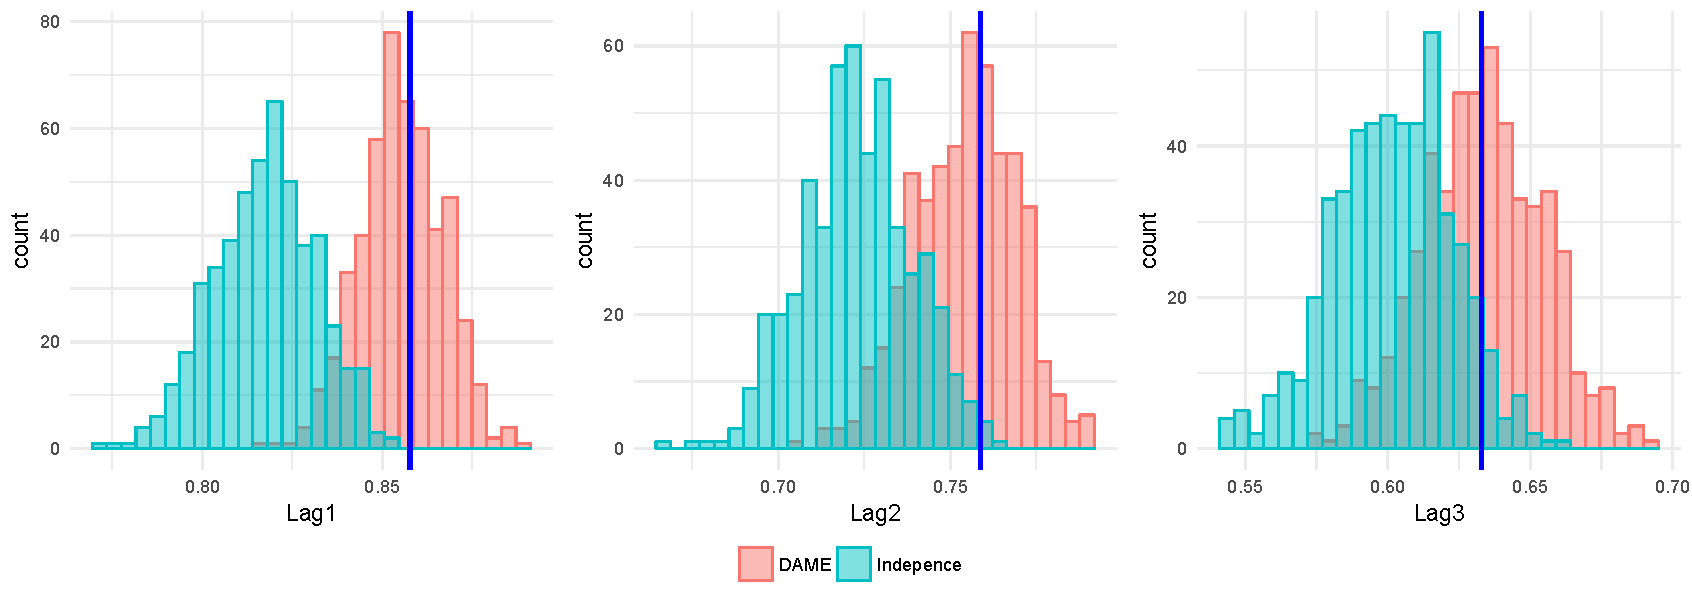
\includegraphics[width=1\textwidth]{plots/correlation_histogram.pdf}	
	\caption {Histogram of posterior lagged degree correlations (from lag 1 to lag 3): the DAME (red) and independence model (blue), with the observed lagged degree correlations (blue lines)}
	\label{figure:correlationstudy}
\end{figure}
\subsection{Capturing Transitivity} \label{subsec: negative transitivity}
Similar to Section \ref{subsec: correlation}, we generated  $\mathbf{Y}$ with $N=20$, $T=10$, $P=1$ (intercept only), $R=2$, and $(a, b) = (2, 1)$ for all inverse-Gamma hyperparameters. On the other hand, considering that our new goal is not to estimate temporal correlations but to represent positive or negative transitivity, this time we modify two settings: 1) set $(\kappa^\beta, \kappa^\theta, \kappa^d) = (0.001, 0.001, 0.001)$ such that all paramters and the resulting dynamic network is nearly independent over time, and 2) force $d^t_{r} > 0$ or $d^t_{r} <0$ for all $r=1,2$ and $t=1,...,10$ such that the generated network exibits positive or negative transitive feature, respectively. Again, we ran 6,000 MCMC iterations and discarded the first 1,000, with thinning = 10, however, we fixed $\kappa$'s at the true values and did not estimate the covariance paramters such that the difference in performance only comes from the multiplicative effects formulations, $u^\prime Du$ and $u^\prime u$. If we estimated $\kappa$'s for this comparison, the difference in results may not only arise from the formulation of multiplicative effects, but also possibly come from lack of correlation structure in $u^\prime u$ because our modeling framework do not assign any correlation on $u$'s.   \\ \newline 
Figure 2 shows a graphical comparison between the two formulations of the multiplicative random effects with respect to the second and third moments of degree (i.e. degree($\hat{Y}^2$) and degree($\hat{Y}^3$), respectively), for a randomly chosen node (node 2). For the case of positive transitivity ($d > 0$), our model and its alternative (without $D$ term) do not show significant differences; both formulations achieve great performance in replicating the first, second, and third moments of node 2's degree. On the contrary, when we fit the network with negative transitivity ($d < 0$), the two formulations reveal noticeable differences. While the DAME can still recover the true degree in all three moments, the model without $D$ term shows inaccuracy in simulating a network that is close to the true data, especially in higher moments. Not only the $u^\prime u$ model introduces bias, but also it shows lower precision than our model. This notable difference strongly supports our argument that $u^\prime Du$ should be preferred over $u^\prime u$, as a standard form of multiplicative random effects.
\begin{figure}[H]
	\centering
			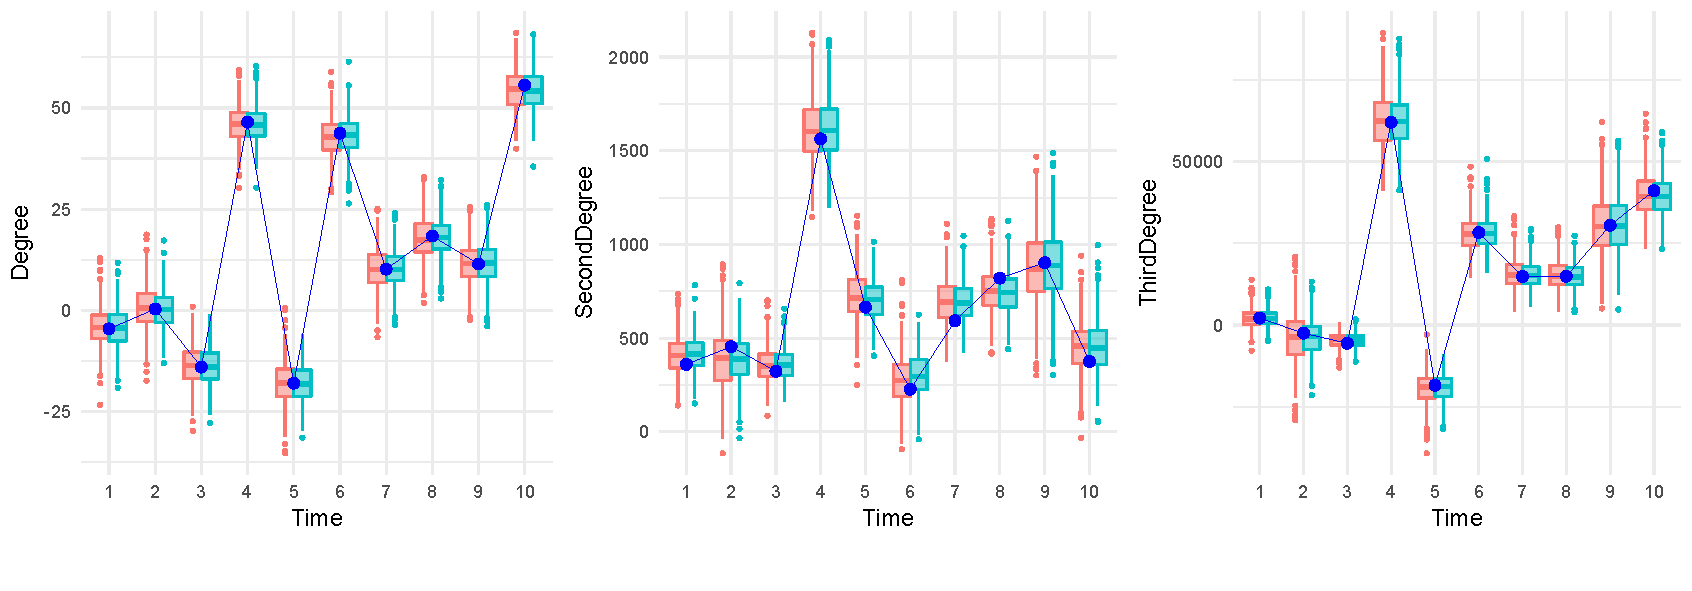
\includegraphics[width=1\textwidth]{plots/Degreeplot.pdf}	
						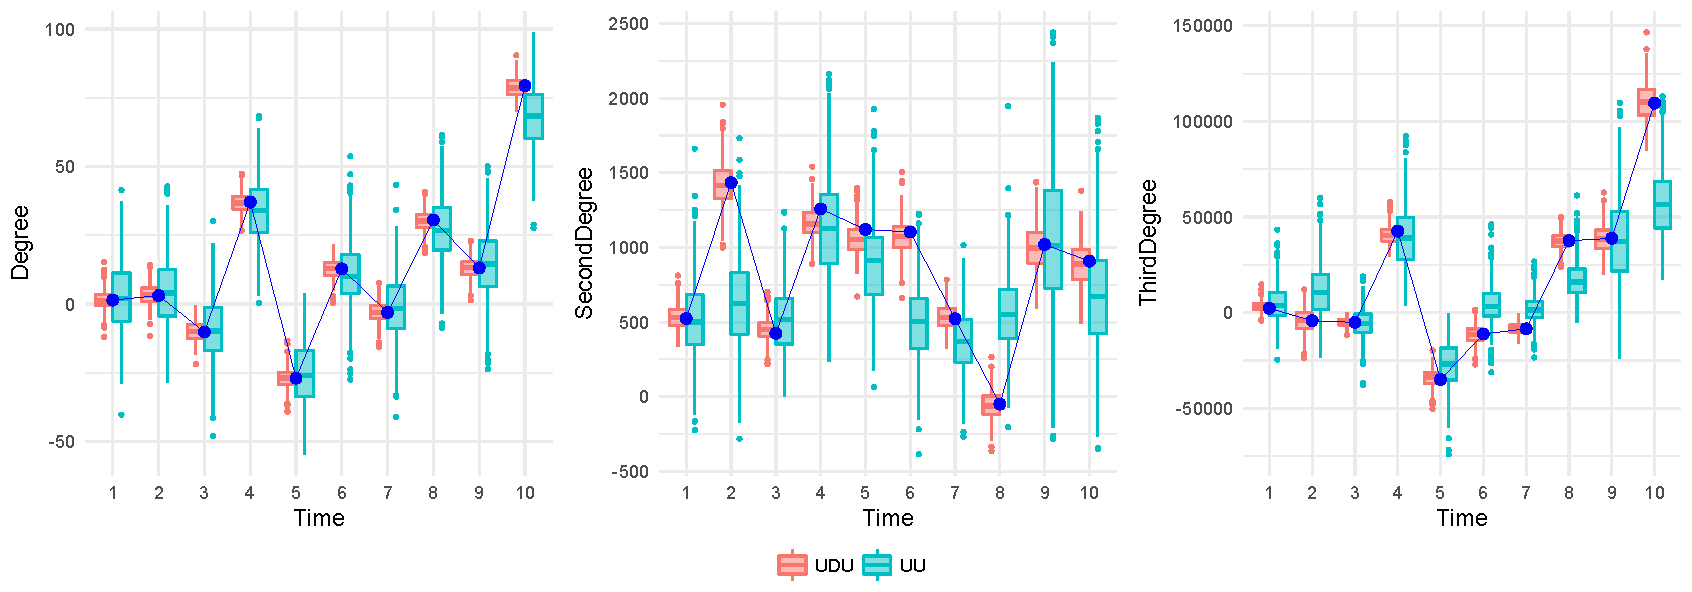
\includegraphics[width=1\textwidth]{plots/Degreeplot2.pdf}	
	\caption {Posterior distribution of the first (left), second (middle), and third (right) moment degrees for node 2 using positive transitive network (upper) and negative transitive network (lower): the DAME (red) and without $D$ model (green), with the observed moment degrees (blue dots)}
	\label{figure:negativitystudy}
\end{figure}
\section{Analysis of the United Nations Voting Network}\label{sec: UNvoting}
\subsection{Data}\label{subsec: data processing}
Votes in the United Nations General Assembly (UNGA) have been analyzed in many political science papers \citep{voeten2000clashes,voeten2004resisting,bearce2007intergovernmental,mattes2015leadership,bailey2017estimating}, and became one of the standard data sources to measure the state preferences. Unfortunately, to our knowledge, the existing studies ignored two important features of the dataset. First, votes are highly correlated across timepoints, because they are the reflections from history. \cite{bailey2017estimating} proposed a dynamic ordinal spatial IRT (item response theory) model and allowed for better inter-temporal comparisons, however, their model limited the temporal dependence to be lag 1 (i.e. Markovian assumption --- votes at time $(t+1)$ is only dependent on votes at time $t$). Second, although the researchers have viewed ``voting" as dyadic behavior and thus used dyadic similarity indicators such as affinity or S scores \citep{gartzke1998kant,signorino1999tau}, to our knowledge, the United Nations voting data has never been analyzed using the dynamic network models. \\ \newline
To overcome the limitations and provide the new insight, we apply the DAME to the voting behavior of 74 countries in the United Nations (UN) General Assembly roll-call votes over the 32 year period, from 1983 through 2014. Full list of the 74 countries included in this analysis and their abbreiviationsare listed in Table \ref{table:importantvotes} in Appendix A. These data were obtained from \cite{12379_2016}, where we use the subset of the votes called `important votes', the votes identified as important by U.S. State Department report Voting Practices in the United Nations. Throughout 1983 to 2014, the number of important votes on average is 12 per year, ranges from 6 to 28. Specifically, we construct the response $\mathbf{Y} = \{Y^1,\ldots, Y^{32}\}$, where each $Y^t$ is $74 \times 74$ matrix, using the variable `agree3unimportant' in the original dataset, which is a voting similarity index (0--1) computed using 3 category vote data (Y = “yes” or approval for an issue; A = abstain; N = “no” or disapproval for an issue)\footnote{voting similarity index between the two countries $i$ and $j$ at year $t$ is calculated as (Number of votes $i$ and $j$ agreed at year $t$) / (Number of votes $i$ and $j$ both participated at year $t$)}. Note that abstention is counted as half-agreement with a yes or no vote, while two abstention is treated as full-agreement. For basic summary of Unite Nations voting data including the average number of common votes and the averge proportion of agreement or voting similarity index per year, see Table \ref{table:EDA} in Appendix B. \\ \newline
As an exploratory data analysis, Table \ref{table:corr} illustrates the lagged degree correlation (defined in Equation (4)) of the dataset, which is used in Section \ref{subsec: correlation}, to measure how much Unite Nations voting data is correlated over time. There exists strong positive correlation in how countries vote in the United Nations General Assembly over time, and as the distance between two timepoints become larger the correlation gets weaker. This provides solid evidence that our model with Gaussian process assumption is one of the appropriate appraoches to effectively analyze this dataset.
\begin{table}[ht]
	\centering
	\begin{tabular}{ |c|c|c|c|c|c|c|c|c|c|c|} 
		\hline
		{Lag}	& 1 & 2& 3& 4& 5& 6& 7&8&9&10 \\ \hline
		Correlation & 0.800&0.745&0.669&0.589&0.541&0.430&0.365&0.246&0.218& 0.203\\\hline
	\end{tabular}
	\caption {Lagged degree correlation of United Nations Voting Data}
	\label{table:corr}
\end{table}
\newline Next, to dynamically model the voting network in relation to other variables reflecting international relations,  we combine $P=5$ different dyadic variables from the Correlates of War (COW) data \citep{gibler2008international}, Polity IV data \citep{marshall2014polity} and the International Monetary Fund (IMF)'s Direction of Trade Statistics (DOTS) and International Financial Statistics (IFS) data, and construct the observed edge covariates $\mathbf{X}$. For every $p=1,...,5$, we set the explanatory variable $X^t_{ijp}$ as below:
\begin{itemize}
	\item [1.] $\mbox{Intercept}^t_{ij}$: constant 1,
	\item [2.] log($\mbox{distance})^t_{ij}$: log of the geographic distance between country $i$ and country $j$,
	\item [3.] $\mbox{Alliance}^t_{ij}$: 1 if country $i$ and country $j$ have alliance, and 0 otherwise,
	\item [4.] $\mbox{Polity difference}^t_{ij}$: absolute difference in polity IV number between country $i$ and country $j$,
	\item [5.] $\mbox{Lower trade-to-GDP ratio}^t_{ij}$: index of economic dependence using bilateral trade weighted by each country's domestic product (GDP), defined in \cite{gartzke2000preferences} $$min\Big(\frac{\mbox{Trade}_{ijt}}{\mbox{GDP}_{it}}, \frac{\mbox{Trade}_{ijt}}{\mbox{GDP}_{jt}}\Big),$$
	\item [6.] $\mbox{Common language}^t_{ij}$: indicator of whether country $i$ and country $j$ share the same language,
\end{itemize}
where all covariates are symmetric $X^t_{ijp}=X^t_{jip}$. Note that intercept is included to account for the baseline degree of agreement at each timepoint. Two variables,  log($\mbox{distance}$) and common language are time-invariant covariates, although their coefficients may vary over time.\\\newline
Moreover, we specified the matrix of availability $A$ introduced in Section \ref{subsec: varying number of nodes} to reflect six countries' nonparticipation in the United Nations Genearl Assembly: 
\begin{itemize}
	\item[1.]  North Korea (PRK) have structural zeros from $t = 1$ to $t = 8$:\\
	- North Korea did not vote until North Korea and South Korea have simultaneously admitted to United Nations in 1991.
	\item[2.] South Korea (ROK) have structural zeros from $t = 1$ to $t = 8$:\\
	- South Korea did not vote until North Korea and South Korea have simultaneously admitted to United Nations in 1991.
	\item [3.] Ukraine (UKR)  has structural zeros from $t=1$ to $t = 9$: \\
	- Previously Ukrainian Soviet Socialist Republic, the country changed its name to Ukraine on 1991 and started voting with new name from 1992.
	\item [4.] Russia (RUS) has structural zeros from $t=1$ to $t =9$:\\
- Russia succeeded the Soviet Union's seat, including its permanent membership on the Security Council in the United Nations after the dissolution of the Soviet Union in 1991. 
	\item [5.] Georgia (GRG) has structural zeros from $t = 1$ to $t = 10$:\\
	-  Georgia, one of the former Soviet Republics, was admitted to United Nations on 1992, thus no voting records until 1992.
	\item [6.] Iraq (IRQ) has structural zeros from $t = 13$ to $t = 21$:\\
	- The country did not participate the UNGA roll-call votes during 1995 - 2003. Since 1990, Iraq was under severe sanctions from the international community including the United Nations.
\end{itemize}
Therefore, any missing values corresponding the country and missing period are treated as structural zeros. In Section \ref{subsec: varying number of nodes}, we mentioned that other non-structural missing values are treated as random missing (and thus imputed), however, this dataset does not include any random missings. 
\subsection{Reduced-Rank Structure of Voting Network}\label{subsec: reduced rank}
In this section, we demonstrate the special low-rank structure of the voting network, which can be generalized into any other similarly constructed agreement networks. First, for simplicity, we assume static network by fixing $T = 1$ and consider the $N \times N$ adjacency matrix $V^1$ representing the network consists of single vote. Since each entry of $V^1$ denotes a voting similarity index (0-1) computed using 3 categories (“yes”, ``abstain", and “no”), the $(i, j)^{th}$ element $V^1_{ij}$ can only have three possible values,
\begin{equation*}
V^1_{ij} =\begin{cases}
1, & \mbox{agreement}\\
0.5, &\mbox{half-agreement (one abstain)}\\
0, & \mbox{disagreement}\\
\end{cases}
\end{equation*}
which implies perfect transitivity of the agreement network, i.e. if there is an agreement between $i$ and $j$, and also between $j$ and $h$, then there must be an agreement between $i$ to $h$, and therefore any two edges sharing one node, such as $V^1_{ij}$ and $V^1_{jh}$, automatically determines the third edge between the unshared nodes $V^1_{ih}$. This constraint makes the maximum rank of $V^1$ to be 3, thus we can use low rank factorization of the matrix $V^1$ using $R=3$. If we were to apply the DAME model to this type of single vote network (without additive effects and explanatory variables), the maximum size of dimension for the latent factors we could fit is $R=3$ and the estimated latent factors can be viewed as the distinct constructs behind the vote. \\ \newline
\iffalse When two votes are aggregated, following the theorem regarding the bounds on the rank of the sum of matrices (modified for symmetric matrices) \citep{marsaglia1967bounds}
\begin{equation*}
 r(A + B) \leq r(A) + r(B) - \mbox{max}(d), 
\end{equation*}
where $r(A)$ is the rank of matrix $A$ and $d = \mbox{dim}(\mathcal{C}_A \cap \mathcal{C}_B)$ with $\mathcal{C}_A$ denoting the column space of $A$, the maximum rank of the matrix $V_1+V_2$ becomes 6. \textcolor{red}{However, due to the perfect transitive constraint of agreement network, $\mbox{max}(d)$ is always greater than 0, thus the maximum rank is 5 in our case.} As a result, we can generalize this finding into the aggregate of $M$ votes:
\begin{equation*}
\mbox{The maximum rank of the matrix $(V_1+V_2,...,V_M)$ is $3 + 2\times (M-1)$,}
\end{equation*}
which is the maximum dimension of latent factors the DAME model could fit, although small value of $R$ (e.g. $R=2$ or $3$) are preferred in general. \fi 
Although it is worth understanding the constraint behind single votes, this is not a practical issue in modeling United Nations voting network, where we aggregate multiple votes per year (minimum number of important votes per year is 6). When we add $M$ number of matrices representing each vote, the aggregated matrix $V^1+V^2+...+V^M$ gets closer to the full rank thus we no longer need to worry about the maximum dimension of the latent factors in fitting the DAME model. Moreover, including the observed covariates $X$ and additive random effects $\theta$ also relax the reduced rank structure, since the multiplicative latent effect $u^\prime Du$ is modeled after we subtract those effects from the response matrix or array (See Section \ref{sec: DAME}). Accounting for large variability in the observed covariates and additive random effects, the residuals no longer maintains the perfect transivity structure.
\subsection{Model Validation}\label{subsec: Model Validation}
To perform a model validation as well as to understand the role of different effects at the same time, we fitted four different dynamic AME models, one with additive and multiplicative effects, one with only multiplicative effects, one with only additive effects, and the last without any random effects, where all four models included 6 fixed effects in Section \ref{subsec: data processing}. We constructed 95\% credible intervals for degree statistics of the model-simulated response $\hat{\mathbf{Y}}$ at every $10^{th}$ sample after burn-in. \\ \newline
Figure \ref{figure:modelvalidation} shows the posterior predictive plots for the country ``Israel" comparing the four models. First of all, there is huge benefit of correcting the bias when we add additive effects, compared to the model with no random effects. Next, when we compare between AE (additive only) and ME (multiplicative only), it is apparent that that the multiplicative effects significantly reduced the interval of estimates. This happens since the additive effects have very small variances ($\approx0$) while the multiplicative effects have larger variance estimates, which significantly lowered the error variance estimates $\hat\sigma_e^2$ that plays a big role in the precision of simulated data. Our model with both additive and multiplicative effects seems to perform similar to the ME model (in this aggregated plot), however, further analysis showed that the DAME still outperform the ME model in terms of both accuracy and precision. Overall, not only the DAME model showed the most accurate estimates over time, but it also had the narrowest 95\% credible intervals among the four. This finding emphasizes the importance of including the additive and multiplicative term in the model, capturing some features not explicable by fixed effects and maximizing model performance. More results using the full DAME model are demonstrated in Section \ref{subsec: UNresult}.
\begin{figure}[H]
	\begin{center}
		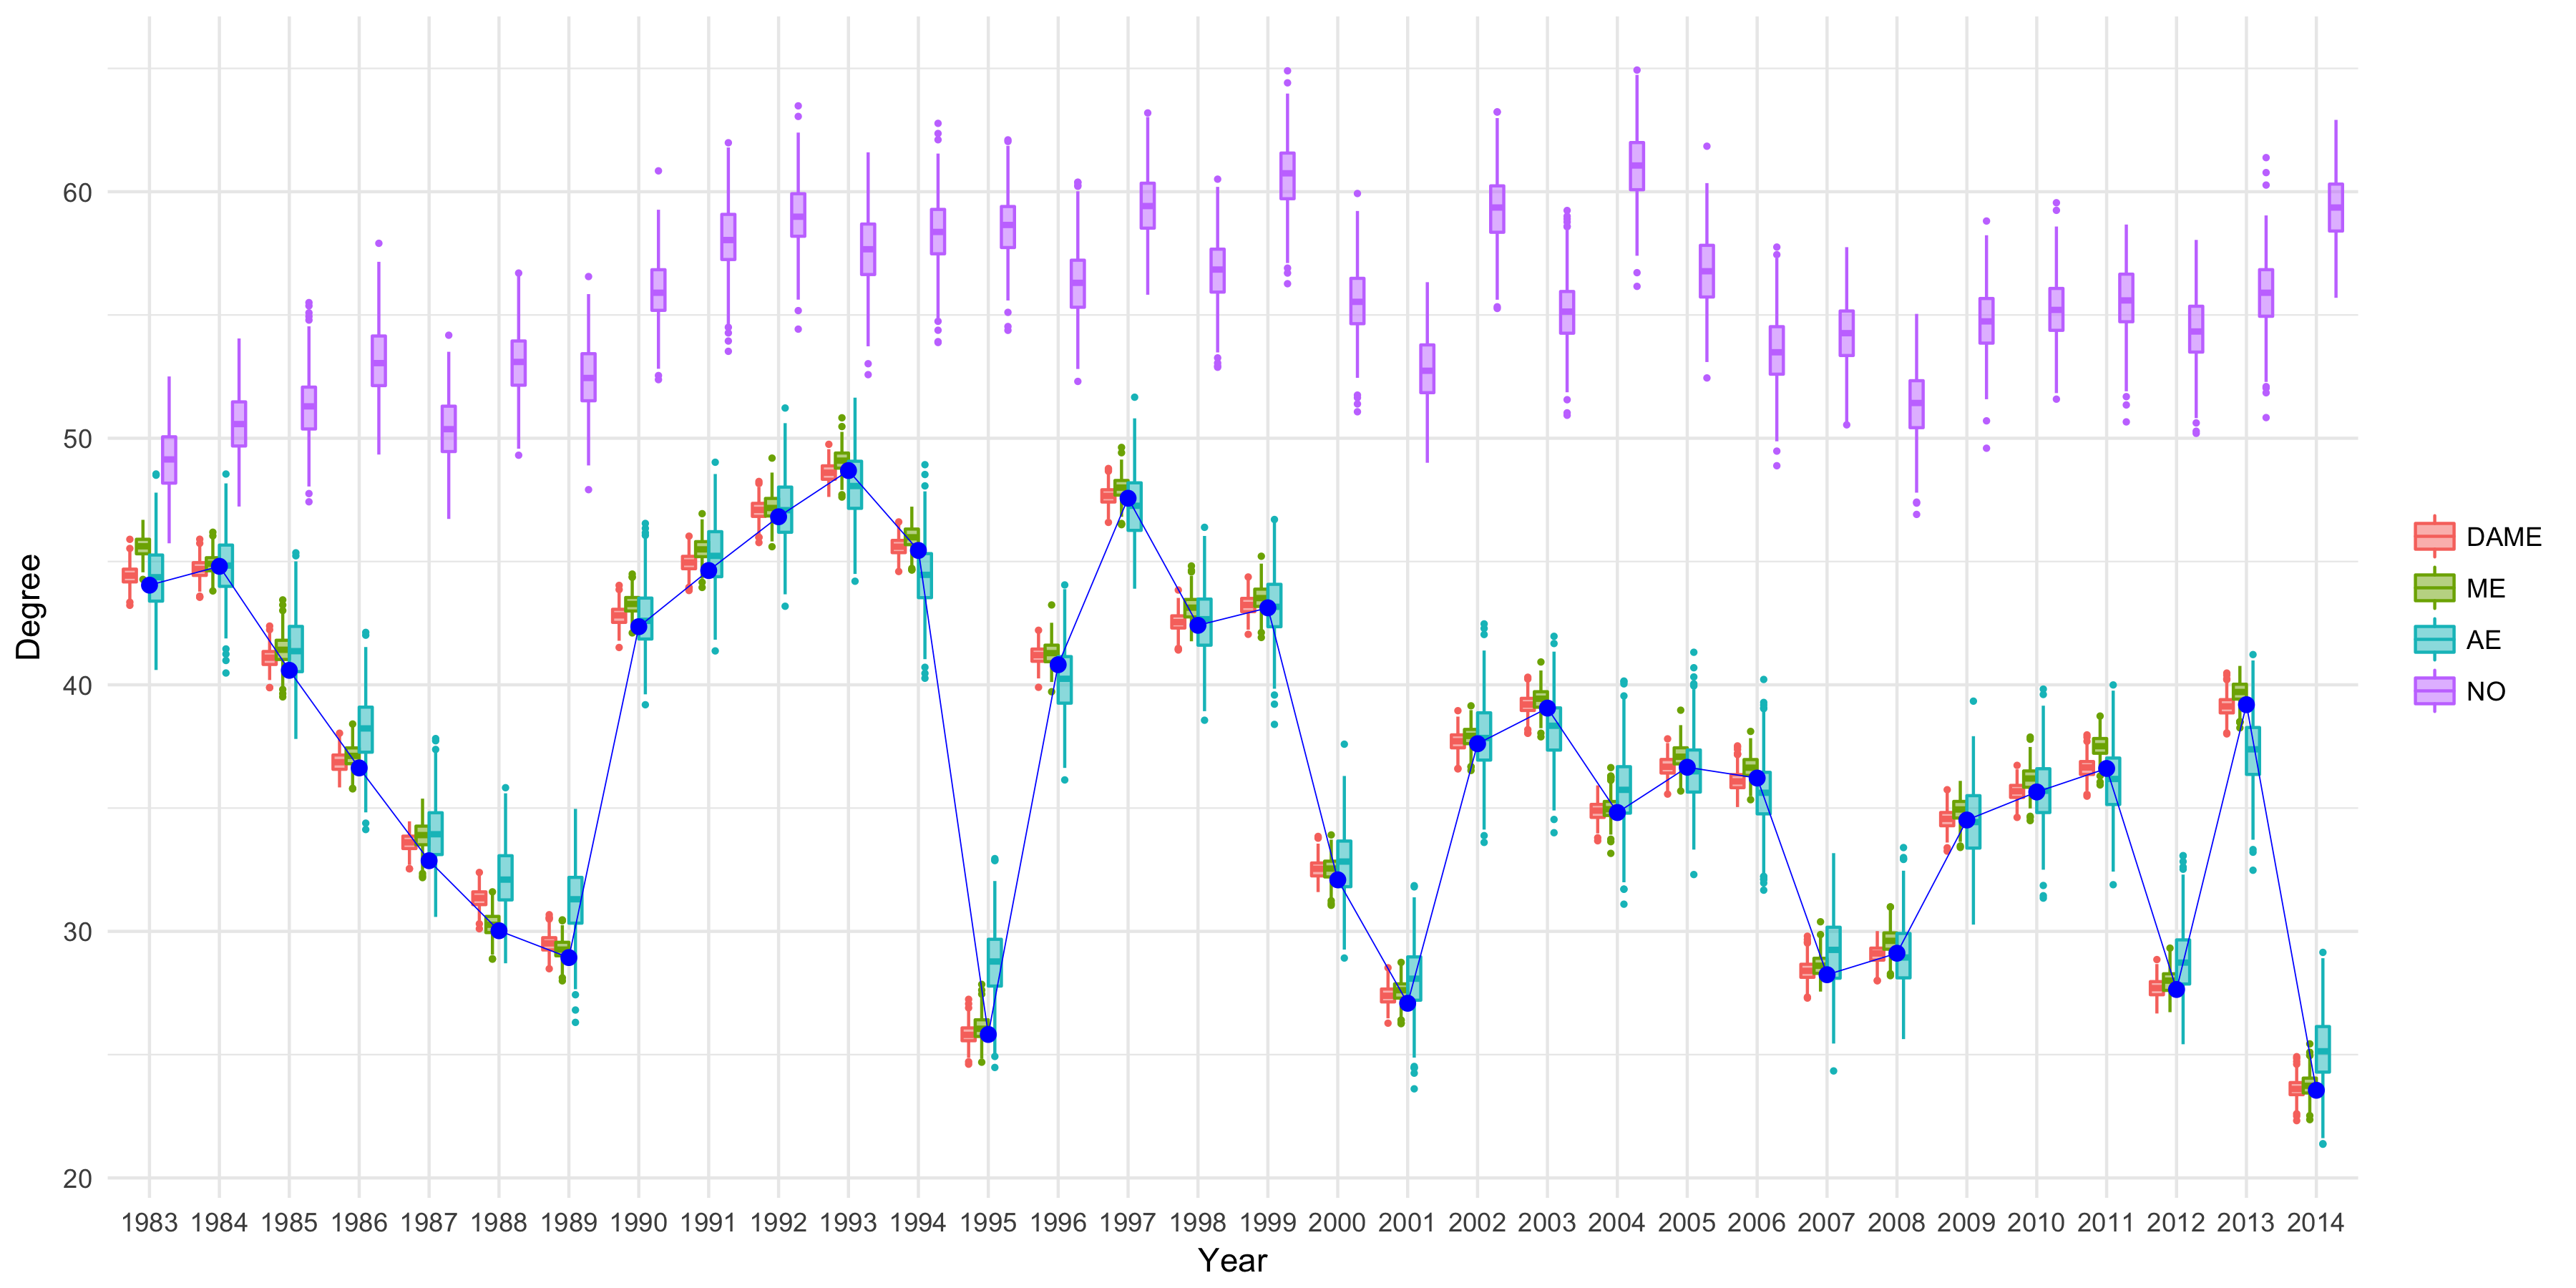
\includegraphics[width=1\textwidth]{plots/ISR31.png}	
	\end{center}
	\caption {Posterior predictive boxplots based on 95\% credible intervals for degree staitstics of Israel (ISR), comparing three models: the DAME (red), only multiplicative effects (green), only additive effects (blue), and no random effects (blue), with the blue dots represent the country's observed degree statistic over 32 years.}
	\label{figure:modelvalidation}
\end{figure}
\subsection{Parameter Estimation and Interpretation}\label{subsec: UNresult}
In this section, we apply the model with the dimension of latent factors chosen as $R=2$, based on some preliminary experiments where increasing the dimension of latent factors did not significantly improve the model fitting. For example, when $R=3$, the last value of estimated eigenvalue $d_{3\cdot}$ is very close to zero for the most of the timepoints $t=1,...,32$. Thus, we present the results from the same settings as Section \ref{subsec: Model Validation}, which are $6,000$ Gibbs iterations with a burn-in of $1,000$, where every $10^{th}$ sample was taken as a thinning. All inverse-Gamma hyperparameters $(a, b) = (2, 1)$, and the covariance parameters $(\kappa, \tau)$ were estimated, following Section \ref{subsec: posterior computation}. Figure \ref{figure:interceptplot} shows the posterior estimates of the fixed effect coefficients $\{\beta_p\}_{p=1}^6$ with their 95\% credible intervals. \textcolor{red}{Interpretation of fixed effect plot} 
\begin{figure}[ht]
	\begin{center}
		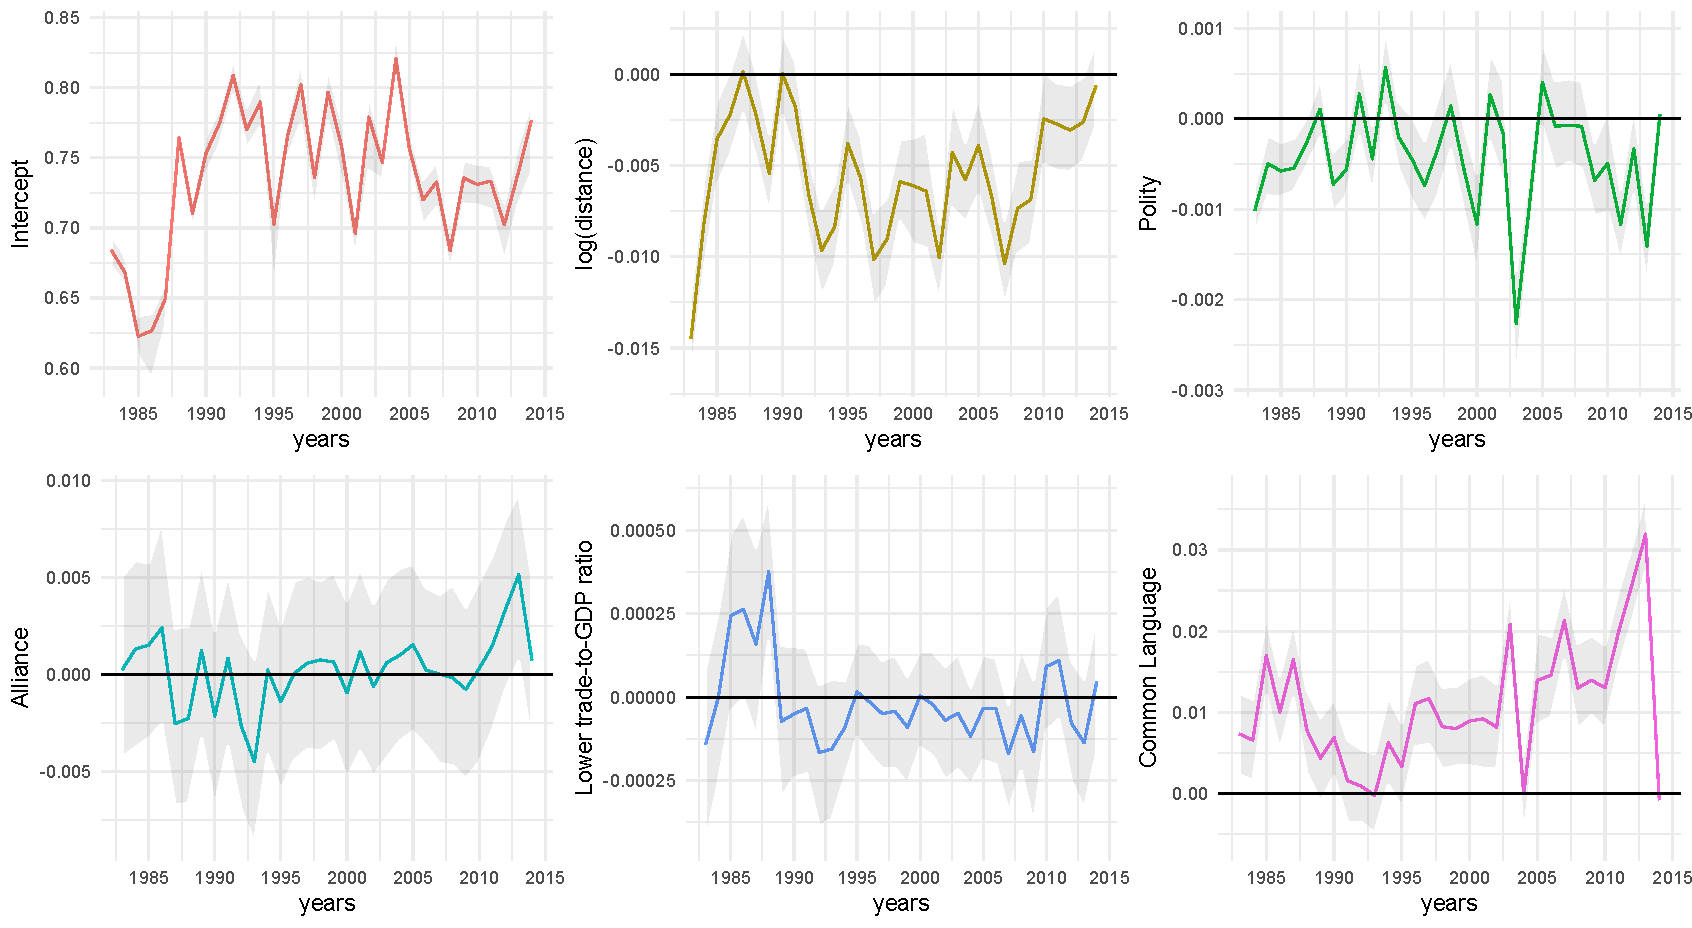
\includegraphics[width=1\textwidth]{plots/betaplot_full.pdf}
	\end{center}
	 	\caption {Posterior mean for the fixed effect coefficients $\{\beta_p\}_{p=1}^6$  (colored line): Intercept, log(distance), Alliance, Polity difference, Lower trade-to-GDP ratio, and Common Language, and their corresponding 95\% credible intervals (grey areas). }
	\label{figure:interceptplot}
\end{figure}
 \newpage
 \begin{figure}[ht]
 	\begin{center}
 		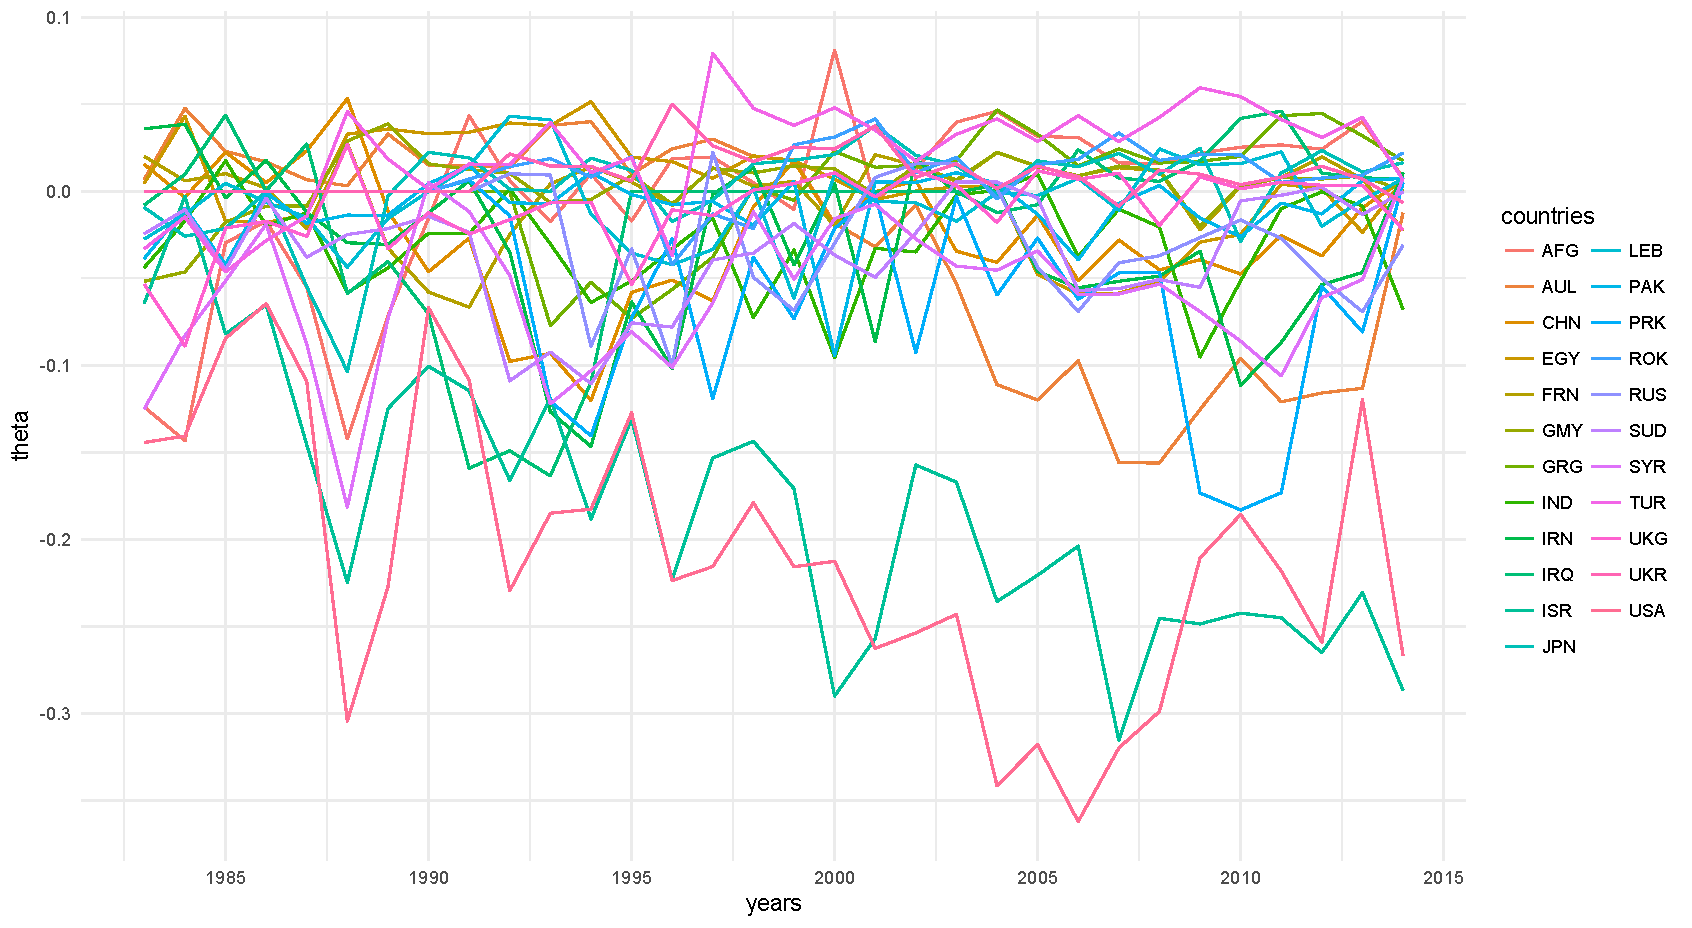
\includegraphics[width=1\textwidth]{plots/theta_reduced.pdf}	
 	\end{center}
 	\caption {Posterior mean estimates for the additive random effect estimates $\theta$.}
 	\label{figure:thetaplot}
 \end{figure}
\noindent After controlling for the observed covariates, we move on to the analysis of random effects, both additive and multiplicative ones. For clear visualization, we only present the results from 23 countries, where the countries are chosen based on the most active countries during the ten year period of 2004 -- 2014 \citep{hoff2015multilinear}. Here, the action types include negative material actions, positive material actions, negative verbal actions and positive verbal actions. The 23 countries are marked with $*$ in Appendix A. Figure \ref{figure:thetaplot} is the posterior mean estimates of each node or country's additive random effects which capture the node-specific and within-dyad dependence. \textcolor{red}{Interpretation of additive random effects}\\ \newpage
\noindent The estimated latent factor coordinates in Figure \ref{figure:UDplot}, which can be viewed as the weighted latent positions of nodes for every 4 years between 1983 and 2014, demonstrate the remaining higher-order network dependencies in United Nations voting behaviors. To determine the posterior estimates of $u$ and $D$ without identifiability issue, we calculated posterior mean of the multiplicative random effect matrix $u^\prime Du$ and applied eigen-decomposition to the posterior mean matrix. $D$ is then the diagonal matrix with eigenvalues, and $u$ becomes the eigenvectors. For this specific plot, we multiplied $d_r$ and $u_{r}$ for each dimension such that the plots reflect the magnitude of eigenvalues.  As mentioned in Section \ref{subsec: reduced rank}, it turned out that none of the eigenvalues were negative, implying that there is no negative transitivity effect in United Nations voting behaviors. \textcolor{red}{Interpretations --- What shoud be said about this multiplicative effect plots?} As illustrated, the model estimated additive and multiplicative latent effects and the movement of latent positions reveal that United Nations voting network reflects interesting and meaningful foreign policy positions and alliance of various countries, even after controlling for other covariates that are considered critical in the international relation studies.
  \begin{figure}[ht]
  	\begin{center}  
  		 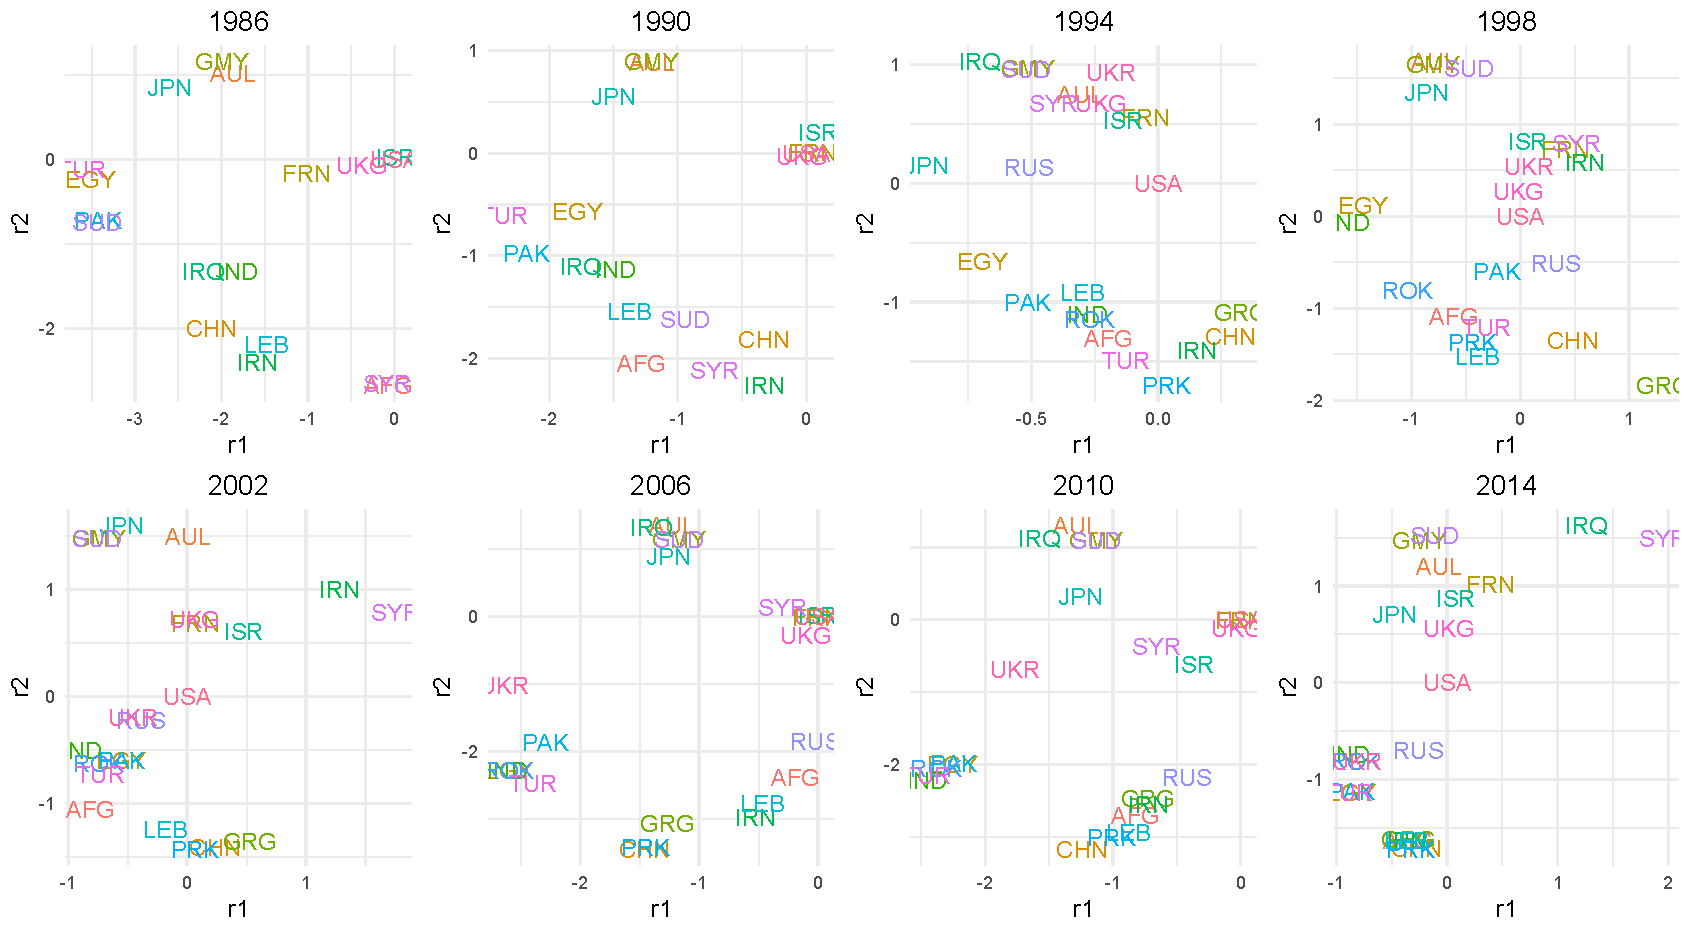
\includegraphics[width=1\textwidth]{plots/UDU_4thyears_reduced.pdf}
  		  		  		    		  	\end{center}
  	\caption {Latent coordinates of the 23 selected countries for every 4 years between 1983 and 2014, obtained from eigen-decomposition of posterior mean of the latent factor matrix $u^\prime Du$. The X-coordinates correspond to $d^t_1\times u^t_{i1}$ and the Y-coordinates correspond to $d^t_2\times u^t_{i2}$.}
  	\label{figure:UDplot}
  \end{figure}
\newpage
\section{Discussion}
Using the correlation associated with network at each time point makes better use of dynamic networks than modeling them as a separate network snapshots. Capturing the temporal dependence from the data is highly informative and should lead to more accurate inference. Our algorithm also eliminates the need to make an arbitrary user-defined covariance structure for determining the prior on the parameters. As a time-varying coefficient extension of the additive and multiplicative effects (AME) model, the dynamic additive and multiplicative nework effects (DAME) model can flexibly learn time-varying network structures, while inferring the effects of latent variables. Further, the visualization of the model estimated time-varying parameters provides an effective temporal trend analysis of dynamic networks, as well as the descriptive visualization of higher-order dependencies from the latent positions over time.
\\\newline
We have demonstrated such effectiveness of our model by modeling the United Nations Voting networks. Although we illustrated the entire framework in the context of symmetric or undirected networks, our model can be easily extended to allow directed networks, following the specification of additive and multiplicative effects model for the directed network \citep{minhas2016inferential}. Furthermore, the approach can be applied to binary and ordinal network data with appropriate link functions, while we currently only provide the application to continuous-valued networks.  Finally, considering the recent explosion of network dataset with extremely large number of nodes or timepoints, our model has a broad range of applicability, suggesting promising computational methods that can accommodate huge networks.
\bibliographystyle{apalike}
\bibliography{BominBib2}
\newpage
\section*{Appendix}
\subsection*{Appendix A: List of Countries in Voting Network}
\begin{table}[H]
	\centering
\begin{tabular}{c|c||c|c}
	\hline
	Abbreviation&Country or area name &	Abbreviation&Country or area name\\
	\hline
			AFG* & Afghanistan & LEB* & Lebanon\\
			ARG& Argentina&MAL&Malaysia\\
			AUL* & Australia&MEX &Mexico \\
			AUS & Austria&MOR & Morocco\\
			BAH & Bahrain&NEW & New Zealand \\
			BNG&  Bangladesh&NIG &      Nigeria\\
			BOL& Bolivia&NOR &Norway \\
			BRA &Brazil&NTH &  Netherlands\\
			BUL & Bulgaria&OMA & Oman\\
				CAN & Canada&PAK* & Pakistan\\
			CAO & Cameroon&PAN & Panama\\
			CHL & Chile&PAR & Paraguay\\
				CHN* & China&PER & Peru\\
				COL & Colombia&PHI & Philippines\\
				COS & Costa Rica&POR & Portugal\\
				CYP & Cyprus&PRK* & North Korea\\
				DEN & Denmark&QAT & Qatar\\
				ECU &Ecuador &ROK* & South Korea\\
				EGY* & Egypt&RUS* & Russia\\
				FIN & Finland&SAU & Saudi Arabia\\
				FRN* & France&SEN &Senegal \\
				GMY* & Germany&SIN &Singapore \\
				GRC & Greece&SPN & Spain\\
				GRG* & Georgia&SRI &   Sri Lanka\\
				GUA &Guatemala&SUD* &Sudan\\
				HON &Honduras&SWD &    Sweden\\
				IND* & India&SYR* & Syrian Arab Republic \\
				INS & Indonesia&THI &   Thailand\\
				IRE & Ireland&TRI & Trinidad and Tobago\\
				IRN* & Iran (Islamic Republic of)&TUN & Tunisia\\
				IRQ* & Iraq&TUR*& Turkey\\
				ISR* & Israel&UAE & United Arab Emirates\\
				ITA & Italy&UKG* & United Kingdom\\
				JOR & Jordan&UKR* & Ukraine\\
				JPN* & Japan&URU & Uruguay\\
				KEN & Kenya&USA* & United States of America\\
				KUW & Kuwait&ZAM & Zambia\\
				\hline
	\label{table:importantvotes}
\end{tabular}
	\caption {List of 74 countries included in the analysis}
\end{table}
\subsection*{Appendix B: Summary of UN Voting Network}
\begin{table}[ht]
	\centering
	\begin{tabular}{ |c|c|c|c|c|c|c|c|c|c|} 
		\hline
		{Year}	& 1983 & 1984& 1985& 1986 & 1987& 1988& 1989&1990&1991\\ \hline
		Joint votes & 7.447&7.501&8.371&9.424&8.532&5.273&13.213&7.557&9.039\\\hline
		Agreement & 0.694& 0.716 & 0.733 & 0.761 & 0.728 & 0.773 & 0.767 & 0.817 & 0.818\\\hline\hline 
		{Year}	& 1992&1993& 1994 & 1995& 1996& 1997 & 1998& 1999& 2000\\ \hline
		Joint votes  &14.424&11.317&13.922&26.541&9.920&10.460&9.105&11.808&9.276\\\hline
		Agreement & 0.804&0.766& 0.785 & 0.814 & 0.763& 0.803 & 0.770& 0.833 & 0.747\\\hline\hline
		{Year}	&2001&2002&2003&2004&2005& 2006& 2007& 2008&  2009\\ \hline
		Joint votes &9.568&13.511&12.538&8.812&9.546&11.467&11.362&11.652&11.602\\\hline
		Agreement &0.706 & 0.805& 0.731& 0.819& 0.754& 0.709& 0.715&0.670&0.721\\
		\hline\hline
		Year & 2010& 2011&2012&2013&2014&&&&\\\hline
		Joint votes&12.678&9.679&7.892&10.758&12.626&&&&\\\hline
		Agreement&  0.722& 0.735& 0.714 &0.739&0.810&&&&\\\hline
	\end{tabular}
	\caption {Summary of United Nations Voting Data: Average number of common votes (upper) and averge proportion of agreement or voting similarity index (lower) per year}
	\label{table:EDA}
\end{table}
\end{document}

